% Created by tikzDevice version 0.12.3 on 2020-09-18 15:56:04
% !TEX encoding = UTF-8 Unicode
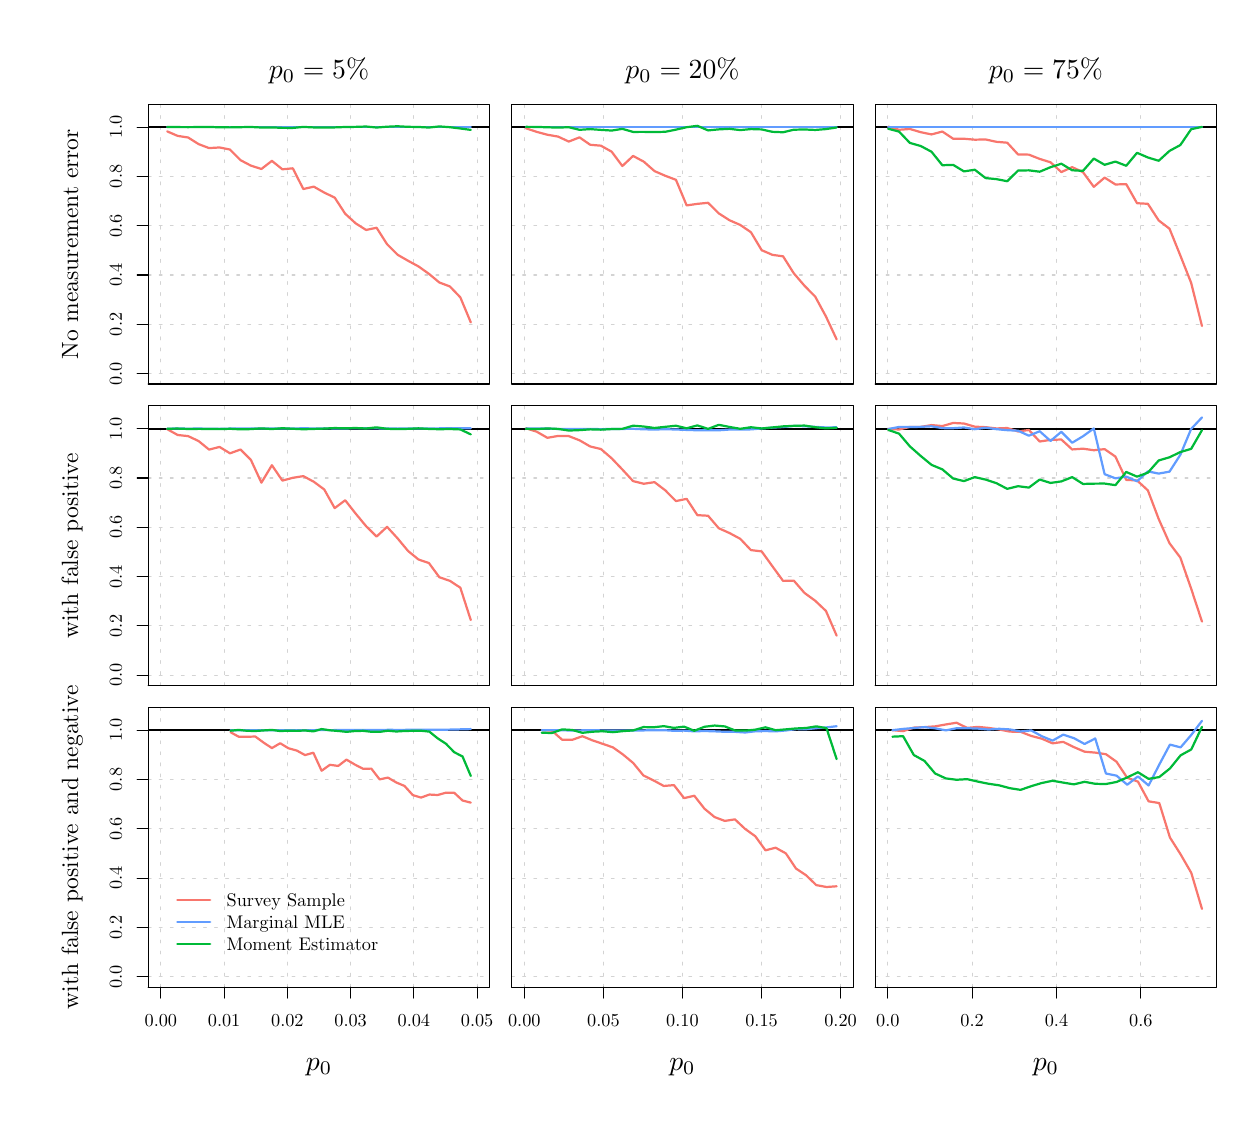
\begin{tikzpicture}[x=1pt,y=1pt]
\definecolor{fillColor}{RGB}{255,255,255}
\path[use as bounding box,fill=fillColor,fill opacity=0.00] (0,0) rectangle (433.62,390.26);
\begin{scope}
\path[clip] ( 39.60,257.53) rectangle (170.94,366.50);
\definecolor{drawColor}{RGB}{0,0,0}

\node[text=drawColor,anchor=base,inner sep=0pt, outer sep=0pt, scale=  0.66] at (105.27,231.40) {Simulation ID};

\node[text=drawColor,rotate= 90.00,anchor=base,inner sep=0pt, outer sep=0pt, scale=  0.66] at ( 18.22,312.01) {Ratio of RMSE};
\end{scope}
\begin{scope}
\path[clip] (  0.00,  0.00) rectangle (433.62,390.26);
\definecolor{drawColor}{RGB}{0,0,0}

\path[draw=drawColor,line width= 0.4pt,line join=round,line cap=round] ( 43.56,265.23) -- ( 43.56,354.34);

\path[draw=drawColor,line width= 0.4pt,line join=round,line cap=round] ( 43.56,265.23) -- ( 39.60,265.23);

\path[draw=drawColor,line width= 0.4pt,line join=round,line cap=round] ( 43.56,283.06) -- ( 39.60,283.06);

\path[draw=drawColor,line width= 0.4pt,line join=round,line cap=round] ( 43.56,300.88) -- ( 39.60,300.88);

\path[draw=drawColor,line width= 0.4pt,line join=round,line cap=round] ( 43.56,318.70) -- ( 39.60,318.70);

\path[draw=drawColor,line width= 0.4pt,line join=round,line cap=round] ( 43.56,336.52) -- ( 39.60,336.52);

\path[draw=drawColor,line width= 0.4pt,line join=round,line cap=round] ( 43.56,354.34) -- ( 39.60,354.34);

\node[text=drawColor,rotate= 90.00,anchor=base,inner sep=0pt, outer sep=0pt, scale=  0.66] at ( 34.06,265.23) {0.0};

\node[text=drawColor,rotate= 90.00,anchor=base,inner sep=0pt, outer sep=0pt, scale=  0.66] at ( 34.06,283.06) {0.2};

\node[text=drawColor,rotate= 90.00,anchor=base,inner sep=0pt, outer sep=0pt, scale=  0.66] at ( 34.06,300.88) {0.4};

\node[text=drawColor,rotate= 90.00,anchor=base,inner sep=0pt, outer sep=0pt, scale=  0.66] at ( 34.06,318.70) {0.6};

\node[text=drawColor,rotate= 90.00,anchor=base,inner sep=0pt, outer sep=0pt, scale=  0.66] at ( 34.06,336.52) {0.8};

\node[text=drawColor,rotate= 90.00,anchor=base,inner sep=0pt, outer sep=0pt, scale=  0.66] at ( 34.06,354.34) {1.0};
\end{scope}
\begin{scope}
\path[clip] ( 43.56,261.49) rectangle (166.98,362.54);
\definecolor{drawColor}{RGB}{211,211,211}

\path[draw=drawColor,line width= 0.4pt,dash pattern=on 1pt off 3pt ,line join=round,line cap=round] ( 48.13,261.49) -- ( 48.13,362.54);

\path[draw=drawColor,line width= 0.4pt,dash pattern=on 1pt off 3pt ,line join=round,line cap=round] ( 70.99,261.49) -- ( 70.99,362.54);

\path[draw=drawColor,line width= 0.4pt,dash pattern=on 1pt off 3pt ,line join=round,line cap=round] ( 93.84,261.49) -- ( 93.84,362.54);

\path[draw=drawColor,line width= 0.4pt,dash pattern=on 1pt off 3pt ,line join=round,line cap=round] (116.70,261.49) -- (116.70,362.54);

\path[draw=drawColor,line width= 0.4pt,dash pattern=on 1pt off 3pt ,line join=round,line cap=round] (139.55,261.49) -- (139.55,362.54);

\path[draw=drawColor,line width= 0.4pt,dash pattern=on 1pt off 3pt ,line join=round,line cap=round] (162.41,261.49) -- (162.41,362.54);

\path[draw=drawColor,line width= 0.4pt,dash pattern=on 1pt off 3pt ,line join=round,line cap=round] ( 43.56,265.23) -- (166.98,265.23);

\path[draw=drawColor,line width= 0.4pt,dash pattern=on 1pt off 3pt ,line join=round,line cap=round] ( 43.56,283.06) -- (166.98,283.06);

\path[draw=drawColor,line width= 0.4pt,dash pattern=on 1pt off 3pt ,line join=round,line cap=round] ( 43.56,300.88) -- (166.98,300.88);

\path[draw=drawColor,line width= 0.4pt,dash pattern=on 1pt off 3pt ,line join=round,line cap=round] ( 43.56,318.70) -- (166.98,318.70);

\path[draw=drawColor,line width= 0.4pt,dash pattern=on 1pt off 3pt ,line join=round,line cap=round] ( 43.56,336.52) -- (166.98,336.52);

\path[draw=drawColor,line width= 0.4pt,dash pattern=on 1pt off 3pt ,line join=round,line cap=round] ( 43.56,354.34) -- (166.98,354.34);
\end{scope}
\begin{scope}
\path[clip] (  0.00,  0.00) rectangle (433.62,390.26);
\definecolor{drawColor}{RGB}{0,0,0}

\path[draw=drawColor,line width= 0.4pt,line join=round,line cap=round] ( 43.56,261.49) --
	(166.98,261.49) --
	(166.98,362.54) --
	( 43.56,362.54) --
	( 43.56,261.49);
\end{scope}
\begin{scope}
\path[clip] ( 43.56,261.49) rectangle (166.98,362.54);
\definecolor{drawColor}{RGB}{0,0,0}

\path[draw=drawColor,line width= 0.8pt,line join=round,line cap=round] ( 43.56,354.34) -- (166.98,354.34);
\definecolor{drawColor}{RGB}{248,118,109}

\path[draw=drawColor,line width= 0.8pt,line join=round,line cap=round] ( 50.42,352.78) --
	( 54.20,351.15) --
	( 57.98,350.57) --
	( 61.77,348.18) --
	( 65.55,346.74) --
	( 69.33,346.97) --
	( 73.11,346.21) --
	( 76.90,342.38) --
	( 80.68,340.40) --
	( 84.46,339.19) --
	( 88.25,342.13) --
	( 92.03,339.08) --
	( 95.81,339.43) --
	( 99.60,331.95) --
	(103.38,332.81) --
	(107.16,330.67) --
	(110.94,328.85) --
	(114.73,323.03) --
	(118.51,319.55) --
	(122.29,317.16) --
	(126.08,317.96) --
	(129.86,312.01) --
	(133.64,308.22) --
	(137.43,306.04) --
	(141.21,303.99) --
	(144.99,301.31) --
	(148.77,298.17) --
	(152.56,296.75) --
	(156.34,292.81) --
	(160.12,283.75);
\definecolor{drawColor}{RGB}{97,156,255}

\path[draw=drawColor,line width= 0.8pt,line join=round,line cap=round] ( 50.42,354.34) --
	( 54.20,354.34) --
	( 57.98,354.34) --
	( 61.77,354.34) --
	( 65.55,354.34) --
	( 69.33,354.34) --
	( 73.11,354.34) --
	( 76.90,354.34) --
	( 80.68,354.34) --
	( 84.46,354.34) --
	( 88.25,354.34) --
	( 92.03,354.34) --
	( 95.81,354.34) --
	( 99.60,354.34) --
	(103.38,354.34) --
	(107.16,354.34) --
	(110.94,354.34) --
	(114.73,354.34) --
	(118.51,354.34) --
	(122.29,354.34) --
	(126.08,354.34) --
	(129.86,354.34) --
	(133.64,354.34) --
	(137.43,354.34) --
	(141.21,354.34) --
	(144.99,354.34) --
	(148.77,354.34) --
	(152.56,354.34) --
	(156.34,354.34) --
	(160.12,354.34);
\definecolor{drawColor}{RGB}{0,186,56}

\path[draw=drawColor,line width= 0.8pt,line join=round,line cap=round] ( 50.42,354.38) --
	( 54.20,354.33) --
	( 57.98,354.31) --
	( 61.77,354.34) --
	( 65.55,354.37) --
	( 69.33,354.27) --
	( 73.11,354.23) --
	( 76.90,354.30) --
	( 80.68,354.37) --
	( 84.46,354.18) --
	( 88.25,354.22) --
	( 92.03,354.05) --
	( 95.81,354.03) --
	( 99.60,354.39) --
	(103.38,354.21) --
	(107.16,354.17) --
	(110.94,354.22) --
	(114.73,354.36) --
	(118.51,354.41) --
	(122.29,354.54) --
	(126.08,354.17) --
	(129.86,354.47) --
	(133.64,354.63) --
	(137.43,354.43) --
	(141.21,354.37) --
	(144.99,354.17) --
	(148.77,354.57) --
	(152.56,354.29) --
	(156.34,353.83) --
	(160.12,353.32);
\end{scope}
\begin{scope}
\path[clip] (  0.00,  0.00) rectangle (433.62,390.26);
\definecolor{drawColor}{RGB}{0,0,0}

\node[text=drawColor,rotate= 90.00,anchor=base,inner sep=0pt, outer sep=0pt, scale=  0.85] at ( 18.22,312.01) {No measurement error};

\node[text=drawColor,anchor=base,inner sep=0pt, outer sep=0pt, scale=  1.00] at (105.27,372.04) {$p_0 = 5\%$};
\end{scope}
\begin{scope}
\path[clip] (170.94,257.53) rectangle (302.28,366.50);
\definecolor{drawColor}{RGB}{0,0,0}

\node[text=drawColor,anchor=base,inner sep=0pt, outer sep=0pt, scale=  0.66] at (236.61,231.40) {Simulation ID};

\node[text=drawColor,rotate= 90.00,anchor=base,inner sep=0pt, outer sep=0pt, scale=  0.66] at (149.56,312.01) {Ratio of RMSE};
\end{scope}
\begin{scope}
\path[clip] (174.90,261.49) rectangle (298.32,362.54);
\definecolor{drawColor}{RGB}{211,211,211}

\path[draw=drawColor,line width= 0.4pt,dash pattern=on 1pt off 3pt ,line join=round,line cap=round] (179.47,261.49) -- (179.47,362.54);

\path[draw=drawColor,line width= 0.4pt,dash pattern=on 1pt off 3pt ,line join=round,line cap=round] (208.04,261.49) -- (208.04,362.54);

\path[draw=drawColor,line width= 0.4pt,dash pattern=on 1pt off 3pt ,line join=round,line cap=round] (236.61,261.49) -- (236.61,362.54);

\path[draw=drawColor,line width= 0.4pt,dash pattern=on 1pt off 3pt ,line join=round,line cap=round] (265.18,261.49) -- (265.18,362.54);

\path[draw=drawColor,line width= 0.4pt,dash pattern=on 1pt off 3pt ,line join=round,line cap=round] (293.75,261.49) -- (293.75,362.54);

\path[draw=drawColor,line width= 0.4pt,dash pattern=on 1pt off 3pt ,line join=round,line cap=round] (174.90,265.23) -- (298.32,265.23);

\path[draw=drawColor,line width= 0.4pt,dash pattern=on 1pt off 3pt ,line join=round,line cap=round] (174.90,283.06) -- (298.32,283.06);

\path[draw=drawColor,line width= 0.4pt,dash pattern=on 1pt off 3pt ,line join=round,line cap=round] (174.90,300.88) -- (298.32,300.88);

\path[draw=drawColor,line width= 0.4pt,dash pattern=on 1pt off 3pt ,line join=round,line cap=round] (174.90,318.70) -- (298.32,318.70);

\path[draw=drawColor,line width= 0.4pt,dash pattern=on 1pt off 3pt ,line join=round,line cap=round] (174.90,336.52) -- (298.32,336.52);

\path[draw=drawColor,line width= 0.4pt,dash pattern=on 1pt off 3pt ,line join=round,line cap=round] (174.90,354.34) -- (298.32,354.34);
\end{scope}
\begin{scope}
\path[clip] (  0.00,  0.00) rectangle (433.62,390.26);
\definecolor{drawColor}{RGB}{0,0,0}

\path[draw=drawColor,line width= 0.4pt,line join=round,line cap=round] (174.90,261.49) --
	(298.32,261.49) --
	(298.32,362.54) --
	(174.90,362.54) --
	(174.90,261.49);
\end{scope}
\begin{scope}
\path[clip] (174.90,261.49) rectangle (298.32,362.54);
\definecolor{drawColor}{RGB}{0,0,0}

\path[draw=drawColor,line width= 0.8pt,line join=round,line cap=round] (174.90,354.34) -- (298.32,354.34);
\definecolor{drawColor}{RGB}{248,118,109}

\path[draw=drawColor,line width= 0.8pt,line join=round,line cap=round] (180.04,353.89) --
	(183.91,352.61) --
	(187.79,351.57) --
	(191.66,350.90) --
	(195.53,349.10) --
	(199.40,350.62) --
	(203.27,347.94) --
	(207.14,347.61) --
	(211.02,345.44) --
	(214.89,340.26) --
	(218.76,343.91) --
	(222.63,341.84) --
	(226.50,338.43) --
	(230.37,336.75) --
	(234.25,335.28) --
	(238.12,326.03) --
	(241.99,326.59) --
	(245.86,326.98) --
	(249.73,323.15) --
	(253.60,320.67) --
	(257.48,318.98) --
	(261.35,316.34) --
	(265.22,309.86) --
	(269.09,308.17) --
	(272.96,307.63) --
	(276.83,301.50) --
	(280.71,296.99) --
	(284.58,293.06) --
	(288.45,285.90) --
	(292.32,277.62);
\definecolor{drawColor}{RGB}{97,156,255}

\path[draw=drawColor,line width= 0.8pt,line join=round,line cap=round] (180.04,354.34) --
	(183.91,354.34) --
	(187.79,354.34) --
	(191.66,354.34) --
	(195.53,354.34) --
	(199.40,354.34) --
	(203.27,354.34) --
	(207.14,354.34) --
	(211.02,354.34) --
	(214.89,354.34) --
	(218.76,354.34) --
	(222.63,354.34) --
	(226.50,354.34) --
	(230.37,354.34) --
	(234.25,354.34) --
	(238.12,354.34) --
	(241.99,354.34) --
	(245.86,354.34) --
	(249.73,354.34) --
	(253.60,354.34) --
	(257.48,354.34) --
	(261.35,354.34) --
	(265.22,354.34) --
	(269.09,354.34) --
	(272.96,354.34) --
	(276.83,354.34) --
	(280.71,354.34) --
	(284.58,354.34) --
	(288.45,354.34) --
	(292.32,354.34);
\definecolor{drawColor}{RGB}{0,186,56}

\path[draw=drawColor,line width= 0.8pt,line join=round,line cap=round] (180.04,354.42) --
	(183.91,354.39) --
	(187.79,354.26) --
	(191.66,354.16) --
	(195.53,354.28) --
	(199.40,353.35) --
	(203.27,353.60) --
	(207.14,353.32) --
	(211.02,353.08) --
	(214.89,353.69) --
	(218.76,352.59) --
	(222.63,352.60) --
	(226.50,352.54) --
	(230.37,352.63) --
	(234.25,353.41) --
	(238.12,354.29) --
	(241.99,354.79) --
	(245.86,353.13) --
	(249.73,353.51) --
	(253.60,353.70) --
	(257.48,353.25) --
	(261.35,353.61) --
	(265.22,353.49) --
	(269.09,352.62) --
	(272.96,352.46) --
	(276.83,353.38) --
	(280.71,353.47) --
	(284.58,353.30) --
	(288.45,353.61) --
	(292.32,354.19);
\end{scope}
\begin{scope}
\path[clip] (  0.00,  0.00) rectangle (433.62,390.26);
\definecolor{drawColor}{RGB}{0,0,0}

\node[text=drawColor,anchor=base,inner sep=0pt, outer sep=0pt, scale=  1.00] at (236.61,372.04) {$p_0 = 20\%$};
\end{scope}
\begin{scope}
\path[clip] (302.28,257.53) rectangle (433.62,366.50);
\definecolor{drawColor}{RGB}{0,0,0}

\node[text=drawColor,anchor=base,inner sep=0pt, outer sep=0pt, scale=  0.66] at (367.95,231.40) {Simulation ID};

\node[text=drawColor,rotate= 90.00,anchor=base,inner sep=0pt, outer sep=0pt, scale=  0.66] at (280.90,312.01) {Ratio of RMSE};
\end{scope}
\begin{scope}
\path[clip] (306.24,261.49) rectangle (429.66,362.54);
\definecolor{drawColor}{RGB}{211,211,211}

\path[draw=drawColor,line width= 0.4pt,dash pattern=on 1pt off 3pt ,line join=round,line cap=round] (310.81,261.49) -- (310.81,362.54);

\path[draw=drawColor,line width= 0.4pt,dash pattern=on 1pt off 3pt ,line join=round,line cap=round] (341.29,261.49) -- (341.29,362.54);

\path[draw=drawColor,line width= 0.4pt,dash pattern=on 1pt off 3pt ,line join=round,line cap=round] (371.76,261.49) -- (371.76,362.54);

\path[draw=drawColor,line width= 0.4pt,dash pattern=on 1pt off 3pt ,line join=round,line cap=round] (402.23,261.49) -- (402.23,362.54);

\path[draw=drawColor,line width= 0.4pt,dash pattern=on 1pt off 3pt ,line join=round,line cap=round] (306.24,265.23) -- (429.66,265.23);

\path[draw=drawColor,line width= 0.4pt,dash pattern=on 1pt off 3pt ,line join=round,line cap=round] (306.24,283.06) -- (429.66,283.06);

\path[draw=drawColor,line width= 0.4pt,dash pattern=on 1pt off 3pt ,line join=round,line cap=round] (306.24,300.88) -- (429.66,300.88);

\path[draw=drawColor,line width= 0.4pt,dash pattern=on 1pt off 3pt ,line join=round,line cap=round] (306.24,318.70) -- (429.66,318.70);

\path[draw=drawColor,line width= 0.4pt,dash pattern=on 1pt off 3pt ,line join=round,line cap=round] (306.24,336.52) -- (429.66,336.52);

\path[draw=drawColor,line width= 0.4pt,dash pattern=on 1pt off 3pt ,line join=round,line cap=round] (306.24,354.34) -- (429.66,354.34);
\end{scope}
\begin{scope}
\path[clip] (  0.00,  0.00) rectangle (433.62,390.26);
\definecolor{drawColor}{RGB}{0,0,0}

\path[draw=drawColor,line width= 0.4pt,line join=round,line cap=round] (306.24,261.49) --
	(429.66,261.49) --
	(429.66,362.54) --
	(306.24,362.54) --
	(306.24,261.49);
\end{scope}
\begin{scope}
\path[clip] (306.24,261.49) rectangle (429.66,362.54);
\definecolor{drawColor}{RGB}{0,0,0}

\path[draw=drawColor,line width= 0.8pt,line join=round,line cap=round] (306.24,354.34) -- (429.66,354.34);
\definecolor{drawColor}{RGB}{248,118,109}

\path[draw=drawColor,line width= 0.8pt,line join=round,line cap=round] (310.96,354.49) --
	(314.87,353.36) --
	(318.78,353.65) --
	(322.69,352.49) --
	(326.60,351.68) --
	(330.51,352.72) --
	(334.42,350.11) --
	(338.33,350.12) --
	(342.24,349.78) --
	(346.15,349.86) --
	(350.05,349.01) --
	(353.96,348.69) --
	(357.87,344.45) --
	(361.78,344.38) --
	(365.69,342.83) --
	(369.60,341.61) --
	(373.51,338.07) --
	(377.42,339.86) --
	(381.33,338.05) --
	(385.24,332.74) --
	(389.15,336.08) --
	(393.05,333.60) --
	(396.96,333.70) --
	(400.87,326.82) --
	(404.78,326.61) --
	(408.69,320.60) --
	(412.60,317.61) --
	(416.51,307.92) --
	(420.42,298.04) --
	(424.33,282.45);
\definecolor{drawColor}{RGB}{97,156,255}

\path[draw=drawColor,line width= 0.8pt,line join=round,line cap=round] (310.96,354.34) --
	(314.87,354.34) --
	(318.78,354.34) --
	(322.69,354.34) --
	(326.60,354.34) --
	(330.51,354.34) --
	(334.42,354.34) --
	(338.33,354.34) --
	(342.24,354.34) --
	(346.15,354.34) --
	(350.05,354.34) --
	(353.96,354.34) --
	(357.87,354.34) --
	(361.78,354.34) --
	(365.69,354.34) --
	(369.60,354.34) --
	(373.51,354.34) --
	(377.42,354.34) --
	(381.33,354.34) --
	(385.24,354.34) --
	(389.15,354.34) --
	(393.05,354.34) --
	(396.96,354.34) --
	(400.87,354.34) --
	(404.78,354.34) --
	(408.69,354.34) --
	(412.60,354.34) --
	(416.51,354.34) --
	(420.42,354.34) --
	(424.33,354.34);
\definecolor{drawColor}{RGB}{0,186,56}

\path[draw=drawColor,line width= 0.8pt,line join=round,line cap=round] (310.96,353.73) --
	(314.87,352.70) --
	(318.78,348.61) --
	(322.69,347.50) --
	(326.60,345.42) --
	(330.51,340.55) --
	(334.42,340.68) --
	(338.33,338.32) --
	(342.24,338.92) --
	(346.15,335.90) --
	(350.05,335.53) --
	(353.96,334.77) --
	(357.87,338.62) --
	(361.78,338.70) --
	(365.69,338.21) --
	(369.60,339.84) --
	(373.51,341.10) --
	(377.42,338.73) --
	(381.33,338.51) --
	(385.24,342.96) --
	(389.15,340.70) --
	(393.05,341.87) --
	(396.96,340.35) --
	(400.87,345.04) --
	(404.78,343.35) --
	(408.69,342.16) --
	(412.60,345.73) --
	(416.51,347.84) --
	(420.42,353.57) --
	(424.33,354.41);
\end{scope}
\begin{scope}
\path[clip] (  0.00,  0.00) rectangle (433.62,390.26);
\definecolor{drawColor}{RGB}{0,0,0}

\node[text=drawColor,anchor=base,inner sep=0pt, outer sep=0pt, scale=  1.00] at (367.95,372.04) {$p_0 = 75\%$};
\end{scope}
\begin{scope}
\path[clip] ( 39.60,148.57) rectangle (170.94,257.53);
\definecolor{drawColor}{RGB}{0,0,0}

\node[text=drawColor,anchor=base,inner sep=0pt, outer sep=0pt, scale=  0.66] at (105.27,122.43) {Simulation ID};

\node[text=drawColor,rotate= 90.00,anchor=base,inner sep=0pt, outer sep=0pt, scale=  0.66] at ( 18.22,203.05) {Ratio of RMSE};
\end{scope}
\begin{scope}
\path[clip] (  0.00,  0.00) rectangle (433.62,390.26);
\definecolor{drawColor}{RGB}{0,0,0}

\path[draw=drawColor,line width= 0.4pt,line join=round,line cap=round] ( 43.56,156.27) -- ( 43.56,245.37);

\path[draw=drawColor,line width= 0.4pt,line join=round,line cap=round] ( 43.56,156.27) -- ( 39.60,156.27);

\path[draw=drawColor,line width= 0.4pt,line join=round,line cap=round] ( 43.56,174.09) -- ( 39.60,174.09);

\path[draw=drawColor,line width= 0.4pt,line join=round,line cap=round] ( 43.56,191.91) -- ( 39.60,191.91);

\path[draw=drawColor,line width= 0.4pt,line join=round,line cap=round] ( 43.56,209.73) -- ( 39.60,209.73);

\path[draw=drawColor,line width= 0.4pt,line join=round,line cap=round] ( 43.56,227.55) -- ( 39.60,227.55);

\path[draw=drawColor,line width= 0.4pt,line join=round,line cap=round] ( 43.56,245.37) -- ( 39.60,245.37);

\node[text=drawColor,rotate= 90.00,anchor=base,inner sep=0pt, outer sep=0pt, scale=  0.66] at ( 34.06,156.27) {0.0};

\node[text=drawColor,rotate= 90.00,anchor=base,inner sep=0pt, outer sep=0pt, scale=  0.66] at ( 34.06,174.09) {0.2};

\node[text=drawColor,rotate= 90.00,anchor=base,inner sep=0pt, outer sep=0pt, scale=  0.66] at ( 34.06,191.91) {0.4};

\node[text=drawColor,rotate= 90.00,anchor=base,inner sep=0pt, outer sep=0pt, scale=  0.66] at ( 34.06,209.73) {0.6};

\node[text=drawColor,rotate= 90.00,anchor=base,inner sep=0pt, outer sep=0pt, scale=  0.66] at ( 34.06,227.55) {0.8};

\node[text=drawColor,rotate= 90.00,anchor=base,inner sep=0pt, outer sep=0pt, scale=  0.66] at ( 34.06,245.37) {1.0};
\end{scope}
\begin{scope}
\path[clip] ( 43.56,152.53) rectangle (166.98,253.57);
\definecolor{drawColor}{RGB}{211,211,211}

\path[draw=drawColor,line width= 0.4pt,dash pattern=on 1pt off 3pt ,line join=round,line cap=round] ( 48.13,152.53) -- ( 48.13,253.57);

\path[draw=drawColor,line width= 0.4pt,dash pattern=on 1pt off 3pt ,line join=round,line cap=round] ( 70.99,152.53) -- ( 70.99,253.57);

\path[draw=drawColor,line width= 0.4pt,dash pattern=on 1pt off 3pt ,line join=round,line cap=round] ( 93.84,152.53) -- ( 93.84,253.57);

\path[draw=drawColor,line width= 0.4pt,dash pattern=on 1pt off 3pt ,line join=round,line cap=round] (116.70,152.53) -- (116.70,253.57);

\path[draw=drawColor,line width= 0.4pt,dash pattern=on 1pt off 3pt ,line join=round,line cap=round] (139.55,152.53) -- (139.55,253.57);

\path[draw=drawColor,line width= 0.4pt,dash pattern=on 1pt off 3pt ,line join=round,line cap=round] (162.41,152.53) -- (162.41,253.57);

\path[draw=drawColor,line width= 0.4pt,dash pattern=on 1pt off 3pt ,line join=round,line cap=round] ( 43.56,156.27) -- (166.98,156.27);

\path[draw=drawColor,line width= 0.4pt,dash pattern=on 1pt off 3pt ,line join=round,line cap=round] ( 43.56,174.09) -- (166.98,174.09);

\path[draw=drawColor,line width= 0.4pt,dash pattern=on 1pt off 3pt ,line join=round,line cap=round] ( 43.56,191.91) -- (166.98,191.91);

\path[draw=drawColor,line width= 0.4pt,dash pattern=on 1pt off 3pt ,line join=round,line cap=round] ( 43.56,209.73) -- (166.98,209.73);

\path[draw=drawColor,line width= 0.4pt,dash pattern=on 1pt off 3pt ,line join=round,line cap=round] ( 43.56,227.55) -- (166.98,227.55);

\path[draw=drawColor,line width= 0.4pt,dash pattern=on 1pt off 3pt ,line join=round,line cap=round] ( 43.56,245.37) -- (166.98,245.37);
\end{scope}
\begin{scope}
\path[clip] (  0.00,  0.00) rectangle (433.62,390.26);
\definecolor{drawColor}{RGB}{0,0,0}

\path[draw=drawColor,line width= 0.4pt,line join=round,line cap=round] ( 43.56,152.53) --
	(166.98,152.53) --
	(166.98,253.57) --
	( 43.56,253.57) --
	( 43.56,152.53);
\end{scope}
\begin{scope}
\path[clip] ( 43.56,152.53) rectangle (166.98,253.57);
\definecolor{drawColor}{RGB}{0,0,0}

\path[draw=drawColor,line width= 0.8pt,line join=round,line cap=round] ( 43.56,245.37) -- (166.98,245.37);
\definecolor{drawColor}{RGB}{248,118,109}

\path[draw=drawColor,line width= 0.8pt,line join=round,line cap=round] ( 50.42,245.18) --
	( 54.20,243.07) --
	( 57.98,242.67) --
	( 61.77,240.88) --
	( 65.55,237.79) --
	( 69.33,238.76) --
	( 73.11,236.45) --
	( 76.90,237.82) --
	( 80.68,234.03) --
	( 84.46,225.83) --
	( 88.25,232.15) --
	( 92.03,226.59) --
	( 95.81,227.60) --
	( 99.60,228.21) --
	(103.38,226.18) --
	(107.16,223.39) --
	(110.94,216.64) --
	(114.73,219.49) --
	(118.51,214.68) --
	(122.29,210.12) --
	(126.08,206.38) --
	(129.86,209.89) --
	(133.64,205.75) --
	(137.43,201.18) --
	(141.21,198.09) --
	(144.99,196.80) --
	(148.77,191.66) --
	(152.56,190.38) --
	(156.34,187.89) --
	(160.12,176.17);
\definecolor{drawColor}{RGB}{97,156,255}

\path[draw=drawColor,line width= 0.8pt,line join=round,line cap=round] ( 50.42,245.36) --
	( 54.20,245.40) --
	( 57.98,245.37) --
	( 61.77,245.39) --
	( 65.55,245.36) --
	( 69.33,245.37) --
	( 73.11,245.38) --
	( 76.90,245.38) --
	( 80.68,245.39) --
	( 84.46,245.40) --
	( 88.25,245.45) --
	( 92.03,245.42) --
	( 95.81,245.41) --
	( 99.60,245.50) --
	(103.38,245.44) --
	(107.16,245.47) --
	(110.94,245.45) --
	(114.73,245.45) --
	(118.51,245.47) --
	(122.29,245.52) --
	(126.08,245.47) --
	(129.86,245.40) --
	(133.64,245.43) --
	(137.43,245.39) --
	(141.21,245.44) --
	(144.99,245.44) --
	(148.77,245.47) --
	(152.56,245.48) --
	(156.34,245.48) --
	(160.12,245.50);
\definecolor{drawColor}{RGB}{0,186,56}

\path[draw=drawColor,line width= 0.8pt,line join=round,line cap=round] ( 50.42,245.34) --
	( 54.20,245.39) --
	( 57.98,245.24) --
	( 61.77,245.28) --
	( 65.55,245.26) --
	( 69.33,245.19) --
	( 73.11,245.31) --
	( 76.90,245.11) --
	( 80.68,245.20) --
	( 84.46,245.47) --
	( 88.25,245.21) --
	( 92.03,245.52) --
	( 95.81,245.32) --
	( 99.60,245.14) --
	(103.38,245.26) --
	(107.16,245.39) --
	(110.94,245.58) --
	(114.73,245.49) --
	(118.51,245.59) --
	(122.29,245.42) --
	(126.08,245.83) --
	(129.86,245.31) --
	(133.64,245.19) --
	(137.43,245.29) --
	(141.21,245.48) --
	(144.99,245.26) --
	(148.77,245.15) --
	(152.56,245.23) --
	(156.34,245.08) --
	(160.12,243.29);
\end{scope}
\begin{scope}
\path[clip] (  0.00,  0.00) rectangle (433.62,390.26);
\definecolor{drawColor}{RGB}{0,0,0}

\node[text=drawColor,rotate= 90.00,anchor=base,inner sep=0pt, outer sep=0pt, scale=  0.85] at ( 18.22,203.05) {with false positive};
\end{scope}
\begin{scope}
\path[clip] (170.94,148.57) rectangle (302.28,257.53);
\definecolor{drawColor}{RGB}{0,0,0}

\node[text=drawColor,anchor=base,inner sep=0pt, outer sep=0pt, scale=  0.66] at (236.61,122.43) {Simulation ID};

\node[text=drawColor,rotate= 90.00,anchor=base,inner sep=0pt, outer sep=0pt, scale=  0.66] at (149.56,203.05) {Ratio of RMSE};
\end{scope}
\begin{scope}
\path[clip] (174.90,152.53) rectangle (298.32,253.57);
\definecolor{drawColor}{RGB}{211,211,211}

\path[draw=drawColor,line width= 0.4pt,dash pattern=on 1pt off 3pt ,line join=round,line cap=round] (179.47,152.53) -- (179.47,253.57);

\path[draw=drawColor,line width= 0.4pt,dash pattern=on 1pt off 3pt ,line join=round,line cap=round] (208.04,152.53) -- (208.04,253.57);

\path[draw=drawColor,line width= 0.4pt,dash pattern=on 1pt off 3pt ,line join=round,line cap=round] (236.61,152.53) -- (236.61,253.57);

\path[draw=drawColor,line width= 0.4pt,dash pattern=on 1pt off 3pt ,line join=round,line cap=round] (265.18,152.53) -- (265.18,253.57);

\path[draw=drawColor,line width= 0.4pt,dash pattern=on 1pt off 3pt ,line join=round,line cap=round] (293.75,152.53) -- (293.75,253.57);

\path[draw=drawColor,line width= 0.4pt,dash pattern=on 1pt off 3pt ,line join=round,line cap=round] (174.90,156.27) -- (298.32,156.27);

\path[draw=drawColor,line width= 0.4pt,dash pattern=on 1pt off 3pt ,line join=round,line cap=round] (174.90,174.09) -- (298.32,174.09);

\path[draw=drawColor,line width= 0.4pt,dash pattern=on 1pt off 3pt ,line join=round,line cap=round] (174.90,191.91) -- (298.32,191.91);

\path[draw=drawColor,line width= 0.4pt,dash pattern=on 1pt off 3pt ,line join=round,line cap=round] (174.90,209.73) -- (298.32,209.73);

\path[draw=drawColor,line width= 0.4pt,dash pattern=on 1pt off 3pt ,line join=round,line cap=round] (174.90,227.55) -- (298.32,227.55);

\path[draw=drawColor,line width= 0.4pt,dash pattern=on 1pt off 3pt ,line join=round,line cap=round] (174.90,245.37) -- (298.32,245.37);
\end{scope}
\begin{scope}
\path[clip] (  0.00,  0.00) rectangle (433.62,390.26);
\definecolor{drawColor}{RGB}{0,0,0}

\path[draw=drawColor,line width= 0.4pt,line join=round,line cap=round] (174.90,152.53) --
	(298.32,152.53) --
	(298.32,253.57) --
	(174.90,253.57) --
	(174.90,152.53);
\end{scope}
\begin{scope}
\path[clip] (174.90,152.53) rectangle (298.32,253.57);
\definecolor{drawColor}{RGB}{0,0,0}

\path[draw=drawColor,line width= 0.8pt,line join=round,line cap=round] (174.90,245.37) -- (298.32,245.37);
\definecolor{drawColor}{RGB}{248,118,109}

\path[draw=drawColor,line width= 0.8pt,line join=round,line cap=round] (180.04,245.51) --
	(183.91,244.27) --
	(187.79,242.06) --
	(191.66,242.72) --
	(195.53,242.67) --
	(199.40,241.16) --
	(203.27,238.92) --
	(207.14,238.00) --
	(211.02,234.65) --
	(214.89,230.60) --
	(218.76,226.41) --
	(222.63,225.45) --
	(226.50,226.03) --
	(230.37,223.10) --
	(234.25,219.19) --
	(238.12,220.00) --
	(241.99,214.11) --
	(245.86,213.89) --
	(249.73,209.37) --
	(253.60,207.64) --
	(257.48,205.56) --
	(261.35,201.48) --
	(265.22,201.01) --
	(269.09,195.66) --
	(272.96,190.35) --
	(276.83,190.45) --
	(280.71,185.99) --
	(284.58,183.17) --
	(288.45,179.50) --
	(292.32,170.56);
\definecolor{drawColor}{RGB}{97,156,255}

\path[draw=drawColor,line width= 0.8pt,line join=round,line cap=round] (180.04,245.42) --
	(183.91,245.42) --
	(187.79,245.41) --
	(191.66,245.24) --
	(195.53,245.25) --
	(199.40,245.23) --
	(203.27,245.26) --
	(207.14,245.18) --
	(211.02,245.23) --
	(214.89,245.26) --
	(218.76,245.31) --
	(222.63,245.12) --
	(226.50,245.05) --
	(230.37,245.15) --
	(234.25,245.06) --
	(238.12,244.90) --
	(241.99,244.78) --
	(245.86,244.78) --
	(249.73,244.77) --
	(253.60,245.04) --
	(257.48,245.04) --
	(261.35,245.10) --
	(265.22,245.43) --
	(269.09,245.73) --
	(272.96,245.95) --
	(276.83,246.37) --
	(280.71,246.24) --
	(284.58,246.00) --
	(288.45,245.80) --
	(292.32,245.85);
\definecolor{drawColor}{RGB}{0,186,56}

\path[draw=drawColor,line width= 0.8pt,line join=round,line cap=round] (180.04,245.30) --
	(183.91,245.20) --
	(187.79,245.44) --
	(191.66,245.27) --
	(195.53,244.68) --
	(199.40,244.83) --
	(203.27,245.11) --
	(207.14,245.00) --
	(211.02,245.21) --
	(214.89,245.29) --
	(218.76,246.43) --
	(222.63,246.13) --
	(226.50,245.61) --
	(230.37,246.02) --
	(234.25,246.42) --
	(238.12,245.49) --
	(241.99,246.54) --
	(245.86,245.28) --
	(249.73,246.74) --
	(253.60,245.98) --
	(257.48,245.31) --
	(261.35,245.88) --
	(265.22,245.43) --
	(269.09,245.80) --
	(272.96,246.19) --
	(276.83,246.38) --
	(280.71,246.48) --
	(284.58,245.88) --
	(288.45,245.47) --
	(292.32,245.69);
\end{scope}
\begin{scope}
\path[clip] (302.28,148.57) rectangle (433.62,257.53);
\definecolor{drawColor}{RGB}{0,0,0}

\node[text=drawColor,anchor=base,inner sep=0pt, outer sep=0pt, scale=  0.66] at (367.95,122.43) {Simulation ID};

\node[text=drawColor,rotate= 90.00,anchor=base,inner sep=0pt, outer sep=0pt, scale=  0.66] at (280.90,203.05) {Ratio of RMSE};
\end{scope}
\begin{scope}
\path[clip] (306.24,152.53) rectangle (429.66,253.57);
\definecolor{drawColor}{RGB}{211,211,211}

\path[draw=drawColor,line width= 0.4pt,dash pattern=on 1pt off 3pt ,line join=round,line cap=round] (310.81,152.53) -- (310.81,253.57);

\path[draw=drawColor,line width= 0.4pt,dash pattern=on 1pt off 3pt ,line join=round,line cap=round] (341.29,152.53) -- (341.29,253.57);

\path[draw=drawColor,line width= 0.4pt,dash pattern=on 1pt off 3pt ,line join=round,line cap=round] (371.76,152.53) -- (371.76,253.57);

\path[draw=drawColor,line width= 0.4pt,dash pattern=on 1pt off 3pt ,line join=round,line cap=round] (402.23,152.53) -- (402.23,253.57);

\path[draw=drawColor,line width= 0.4pt,dash pattern=on 1pt off 3pt ,line join=round,line cap=round] (306.24,156.27) -- (429.66,156.27);

\path[draw=drawColor,line width= 0.4pt,dash pattern=on 1pt off 3pt ,line join=round,line cap=round] (306.24,174.09) -- (429.66,174.09);

\path[draw=drawColor,line width= 0.4pt,dash pattern=on 1pt off 3pt ,line join=round,line cap=round] (306.24,191.91) -- (429.66,191.91);

\path[draw=drawColor,line width= 0.4pt,dash pattern=on 1pt off 3pt ,line join=round,line cap=round] (306.24,209.73) -- (429.66,209.73);

\path[draw=drawColor,line width= 0.4pt,dash pattern=on 1pt off 3pt ,line join=round,line cap=round] (306.24,227.55) -- (429.66,227.55);

\path[draw=drawColor,line width= 0.4pt,dash pattern=on 1pt off 3pt ,line join=round,line cap=round] (306.24,245.37) -- (429.66,245.37);
\end{scope}
\begin{scope}
\path[clip] (  0.00,  0.00) rectangle (433.62,390.26);
\definecolor{drawColor}{RGB}{0,0,0}

\path[draw=drawColor,line width= 0.4pt,line join=round,line cap=round] (306.24,152.53) --
	(429.66,152.53) --
	(429.66,253.57) --
	(306.24,253.57) --
	(306.24,152.53);
\end{scope}
\begin{scope}
\path[clip] (306.24,152.53) rectangle (429.66,253.57);
\definecolor{drawColor}{RGB}{0,0,0}

\path[draw=drawColor,line width= 0.8pt,line join=round,line cap=round] (306.24,245.37) -- (429.66,245.37);
\definecolor{drawColor}{RGB}{248,118,109}

\path[draw=drawColor,line width= 0.8pt,line join=round,line cap=round] (310.96,245.27) --
	(314.87,245.06) --
	(318.78,246.01) --
	(322.69,246.00) --
	(326.60,246.65) --
	(330.51,246.30) --
	(334.42,247.42) --
	(338.33,247.22) --
	(342.24,246.08) --
	(346.15,245.90) --
	(350.05,245.44) --
	(353.96,245.59) --
	(357.87,244.35) --
	(361.78,244.88) --
	(365.69,240.72) --
	(369.60,241.30) --
	(373.51,241.44) --
	(377.42,237.85) --
	(381.33,238.13) --
	(385.24,237.56) --
	(389.15,237.96) --
	(393.05,235.27) --
	(396.96,226.85) --
	(400.87,226.65) --
	(404.78,223.05) --
	(408.69,212.71) --
	(412.60,203.95) --
	(416.51,198.77) --
	(420.42,187.55) --
	(424.33,175.65);
\definecolor{drawColor}{RGB}{97,156,255}

\path[draw=drawColor,line width= 0.8pt,line join=round,line cap=round] (310.96,245.22) --
	(314.87,245.98) --
	(318.78,245.97) --
	(322.69,246.01) --
	(326.60,246.21) --
	(330.51,245.55) --
	(334.42,245.53) --
	(338.33,245.78) --
	(342.24,245.17) --
	(346.15,245.68) --
	(350.05,245.18) --
	(353.96,244.81) --
	(357.87,244.62) --
	(361.78,242.81) --
	(365.69,244.43) --
	(369.60,240.93) --
	(373.51,244.23) --
	(377.42,240.27) --
	(381.33,242.61) --
	(385.24,245.44) --
	(389.15,228.91) --
	(393.05,227.42) --
	(396.96,228.03) --
	(400.87,226.35) --
	(404.78,229.92) --
	(408.69,229.13) --
	(412.60,229.83) --
	(416.51,235.91) --
	(420.42,245.26) --
	(424.33,249.42);
\definecolor{drawColor}{RGB}{0,186,56}

\path[draw=drawColor,line width= 0.8pt,line join=round,line cap=round] (310.96,244.90) --
	(314.87,243.56) --
	(318.78,238.96) --
	(322.69,235.50) --
	(326.60,232.28) --
	(330.51,230.65) --
	(334.42,227.34) --
	(338.33,226.41) --
	(342.24,227.86) --
	(346.15,226.95) --
	(350.05,225.66) --
	(353.96,223.61) --
	(357.87,224.57) --
	(361.78,224.07) --
	(365.69,226.97) --
	(369.60,225.75) --
	(373.51,226.30) --
	(377.42,227.85) --
	(381.33,225.38) --
	(385.24,225.49) --
	(389.15,225.52) --
	(393.05,224.95) --
	(396.96,229.72) --
	(400.87,228.02) --
	(404.78,229.46) --
	(408.69,233.87) --
	(412.60,235.02) --
	(416.51,236.90) --
	(420.42,238.06) --
	(424.33,244.81);
\end{scope}
\begin{scope}
\path[clip] ( 39.60, 39.60) rectangle (170.94,148.57);
\definecolor{drawColor}{RGB}{0,0,0}

\node[text=drawColor,anchor=base,inner sep=0pt, outer sep=0pt, scale=  0.66] at (105.27, 13.46) {Simulation ID};

\node[text=drawColor,rotate= 90.00,anchor=base,inner sep=0pt, outer sep=0pt, scale=  0.66] at ( 18.22, 94.08) {Ratio of RMSE};
\end{scope}
\begin{scope}
\path[clip] (  0.00,  0.00) rectangle (433.62,390.26);
\definecolor{drawColor}{RGB}{0,0,0}

\path[draw=drawColor,line width= 0.4pt,line join=round,line cap=round] ( 43.56, 47.30) -- ( 43.56,136.41);

\path[draw=drawColor,line width= 0.4pt,line join=round,line cap=round] ( 43.56, 47.30) -- ( 39.60, 47.30);

\path[draw=drawColor,line width= 0.4pt,line join=round,line cap=round] ( 43.56, 65.12) -- ( 39.60, 65.12);

\path[draw=drawColor,line width= 0.4pt,line join=round,line cap=round] ( 43.56, 82.94) -- ( 39.60, 82.94);

\path[draw=drawColor,line width= 0.4pt,line join=round,line cap=round] ( 43.56,100.77) -- ( 39.60,100.77);

\path[draw=drawColor,line width= 0.4pt,line join=round,line cap=round] ( 43.56,118.59) -- ( 39.60,118.59);

\path[draw=drawColor,line width= 0.4pt,line join=round,line cap=round] ( 43.56,136.41) -- ( 39.60,136.41);

\node[text=drawColor,rotate= 90.00,anchor=base,inner sep=0pt, outer sep=0pt, scale=  0.66] at ( 34.06, 47.30) {0.0};

\node[text=drawColor,rotate= 90.00,anchor=base,inner sep=0pt, outer sep=0pt, scale=  0.66] at ( 34.06, 65.12) {0.2};

\node[text=drawColor,rotate= 90.00,anchor=base,inner sep=0pt, outer sep=0pt, scale=  0.66] at ( 34.06, 82.94) {0.4};

\node[text=drawColor,rotate= 90.00,anchor=base,inner sep=0pt, outer sep=0pt, scale=  0.66] at ( 34.06,100.77) {0.6};

\node[text=drawColor,rotate= 90.00,anchor=base,inner sep=0pt, outer sep=0pt, scale=  0.66] at ( 34.06,118.59) {0.8};

\node[text=drawColor,rotate= 90.00,anchor=base,inner sep=0pt, outer sep=0pt, scale=  0.66] at ( 34.06,136.41) {1.0};
\end{scope}
\begin{scope}
\path[clip] ( 43.56, 43.56) rectangle (166.98,144.61);
\definecolor{drawColor}{RGB}{211,211,211}

\path[draw=drawColor,line width= 0.4pt,dash pattern=on 1pt off 3pt ,line join=round,line cap=round] ( 48.13, 43.56) -- ( 48.13,144.61);

\path[draw=drawColor,line width= 0.4pt,dash pattern=on 1pt off 3pt ,line join=round,line cap=round] ( 70.99, 43.56) -- ( 70.99,144.61);

\path[draw=drawColor,line width= 0.4pt,dash pattern=on 1pt off 3pt ,line join=round,line cap=round] ( 93.84, 43.56) -- ( 93.84,144.61);

\path[draw=drawColor,line width= 0.4pt,dash pattern=on 1pt off 3pt ,line join=round,line cap=round] (116.70, 43.56) -- (116.70,144.61);

\path[draw=drawColor,line width= 0.4pt,dash pattern=on 1pt off 3pt ,line join=round,line cap=round] (139.55, 43.56) -- (139.55,144.61);

\path[draw=drawColor,line width= 0.4pt,dash pattern=on 1pt off 3pt ,line join=round,line cap=round] (162.41, 43.56) -- (162.41,144.61);

\path[draw=drawColor,line width= 0.4pt,dash pattern=on 1pt off 3pt ,line join=round,line cap=round] ( 43.56, 47.30) -- (166.98, 47.30);

\path[draw=drawColor,line width= 0.4pt,dash pattern=on 1pt off 3pt ,line join=round,line cap=round] ( 43.56, 65.12) -- (166.98, 65.12);

\path[draw=drawColor,line width= 0.4pt,dash pattern=on 1pt off 3pt ,line join=round,line cap=round] ( 43.56, 82.94) -- (166.98, 82.94);

\path[draw=drawColor,line width= 0.4pt,dash pattern=on 1pt off 3pt ,line join=round,line cap=round] ( 43.56,100.77) -- (166.98,100.77);

\path[draw=drawColor,line width= 0.4pt,dash pattern=on 1pt off 3pt ,line join=round,line cap=round] ( 43.56,118.59) -- (166.98,118.59);

\path[draw=drawColor,line width= 0.4pt,dash pattern=on 1pt off 3pt ,line join=round,line cap=round] ( 43.56,136.41) -- (166.98,136.41);
\end{scope}
\begin{scope}
\path[clip] (  0.00,  0.00) rectangle (433.62,390.26);
\definecolor{drawColor}{RGB}{0,0,0}

\path[draw=drawColor,line width= 0.4pt,line join=round,line cap=round] ( 43.56, 43.56) --
	(166.98, 43.56) --
	(166.98,144.61) --
	( 43.56,144.61) --
	( 43.56, 43.56);

\path[draw=drawColor,line width= 0.4pt,line join=round,line cap=round] ( 48.13, 43.56) -- (162.41, 43.56);

\path[draw=drawColor,line width= 0.4pt,line join=round,line cap=round] ( 48.13, 43.56) -- ( 48.13, 39.60);

\path[draw=drawColor,line width= 0.4pt,line join=round,line cap=round] ( 70.99, 43.56) -- ( 70.99, 39.60);

\path[draw=drawColor,line width= 0.4pt,line join=round,line cap=round] ( 93.84, 43.56) -- ( 93.84, 39.60);

\path[draw=drawColor,line width= 0.4pt,line join=round,line cap=round] (116.70, 43.56) -- (116.70, 39.60);

\path[draw=drawColor,line width= 0.4pt,line join=round,line cap=round] (139.55, 43.56) -- (139.55, 39.60);

\path[draw=drawColor,line width= 0.4pt,line join=round,line cap=round] (162.41, 43.56) -- (162.41, 39.60);

\node[text=drawColor,anchor=base,inner sep=0pt, outer sep=0pt, scale=  0.66] at ( 48.13, 29.30) {0.00};

\node[text=drawColor,anchor=base,inner sep=0pt, outer sep=0pt, scale=  0.66] at ( 70.99, 29.30) {0.01};

\node[text=drawColor,anchor=base,inner sep=0pt, outer sep=0pt, scale=  0.66] at ( 93.84, 29.30) {0.02};

\node[text=drawColor,anchor=base,inner sep=0pt, outer sep=0pt, scale=  0.66] at (116.70, 29.30) {0.03};

\node[text=drawColor,anchor=base,inner sep=0pt, outer sep=0pt, scale=  0.66] at (139.55, 29.30) {0.04};

\node[text=drawColor,anchor=base,inner sep=0pt, outer sep=0pt, scale=  0.66] at (162.41, 29.30) {0.05};
\end{scope}
\begin{scope}
\path[clip] ( 43.56, 43.56) rectangle (166.98,144.61);
\definecolor{drawColor}{RGB}{0,0,0}

\path[draw=drawColor,line width= 0.8pt,line join=round,line cap=round] ( 43.56,136.41) -- (166.98,136.41);
\definecolor{drawColor}{RGB}{248,118,109}

\path[draw=drawColor,line width= 0.8pt,line join=round,line cap=round] ( 73.27,135.69) --
	( 76.27,134.03) --
	( 79.26,134.03) --
	( 82.26,134.11) --
	( 85.25,131.92) --
	( 88.25,129.94) --
	( 91.24,131.69) --
	( 94.24,129.87) --
	( 97.23,129.05) --
	(100.23,127.41) --
	(103.22,128.26) --
	(106.22,121.75) --
	(109.21,123.90) --
	(112.21,123.48) --
	(115.20,125.77) --
	(118.20,124.00) --
	(121.19,122.46) --
	(124.18,122.52) --
	(127.18,118.62) --
	(130.17,119.28) --
	(133.17,117.52) --
	(136.16,116.26) --
	(139.16,112.95) --
	(142.15,112.05) --
	(145.15,113.15) --
	(148.14,112.98) --
	(151.14,113.82) --
	(154.13,113.79) --
	(157.13,111.00) --
	(160.12,110.22);
\definecolor{drawColor}{RGB}{97,156,255}

\path[draw=drawColor,line width= 0.8pt,line join=round,line cap=round] ( 73.27,136.41) --
	( 76.27,136.41) --
	( 79.26,136.41) --
	( 82.26,136.42) --
	( 85.25,136.42) --
	( 88.25,136.41) --
	( 91.24,136.40) --
	( 94.24,136.41) --
	( 97.23,136.43) --
	(100.23,136.40) --
	(103.22,136.42) --
	(106.22,136.47) --
	(109.21,136.42) --
	(112.21,136.45) --
	(115.20,136.45) --
	(118.20,136.44) --
	(121.19,136.49) --
	(124.18,136.48) --
	(127.18,136.48) --
	(130.17,136.53) --
	(133.17,136.52) --
	(136.16,136.52) --
	(139.16,136.56) --
	(142.15,136.57) --
	(145.15,136.55) --
	(148.14,136.56) --
	(151.14,136.59) --
	(154.13,136.64) --
	(157.13,136.73) --
	(160.12,136.80);
\definecolor{drawColor}{RGB}{0,186,56}

\path[draw=drawColor,line width= 0.8pt,line join=round,line cap=round] ( 73.27,136.22) --
	( 76.27,136.50) --
	( 79.26,136.19) --
	( 82.26,136.10) --
	( 85.25,136.32) --
	( 88.25,136.51) --
	( 91.24,136.09) --
	( 94.24,136.23) --
	( 97.23,136.15) --
	(100.23,136.31) --
	(103.22,135.97) --
	(106.22,136.81) --
	(109.21,136.36) --
	(112.21,136.12) --
	(115.20,135.81) --
	(118.20,136.09) --
	(121.19,136.17) --
	(124.18,135.83) --
	(127.18,135.80) --
	(130.17,136.21) --
	(133.17,135.93) --
	(136.16,136.11) --
	(139.16,136.18) --
	(142.15,136.20) --
	(145.15,135.89) --
	(148.14,133.46) --
	(151.14,131.51) --
	(154.13,128.45) --
	(157.13,126.91) --
	(160.12,119.87);
\end{scope}
\begin{scope}
\path[clip] (  0.00,  0.00) rectangle (433.62,390.26);
\definecolor{drawColor}{RGB}{0,0,0}

\node[text=drawColor,rotate= 90.00,anchor=base,inner sep=0pt, outer sep=0pt, scale=  0.85] at ( 18.22, 94.08) {with false positive and negative};

\node[text=drawColor,anchor=base,inner sep=0pt, outer sep=0pt, scale=  1.00] at (105.27, 13.46) {$p_0$};
\end{scope}
\begin{scope}
\path[clip] ( 43.56, 43.56) rectangle (166.98,144.61);
\definecolor{drawColor}{RGB}{248,118,109}

\path[draw=drawColor,line width= 0.8pt,line join=round,line cap=round] ( 54.07, 75.02) -- ( 65.95, 75.02);
\definecolor{drawColor}{RGB}{97,156,255}

\path[draw=drawColor,line width= 0.8pt,line join=round,line cap=round] ( 54.07, 67.10) -- ( 65.95, 67.10);
\definecolor{drawColor}{RGB}{0,186,56}

\path[draw=drawColor,line width= 0.8pt,line join=round,line cap=round] ( 54.07, 59.18) -- ( 65.95, 59.18);
\definecolor{drawColor}{RGB}{0,0,0}

\node[text=drawColor,anchor=base west,inner sep=0pt, outer sep=0pt, scale=  0.66] at ( 71.89, 72.75) {Survey Sample};

\node[text=drawColor,anchor=base west,inner sep=0pt, outer sep=0pt, scale=  0.66] at ( 71.89, 64.83) {Marginal MLE};

\node[text=drawColor,anchor=base west,inner sep=0pt, outer sep=0pt, scale=  0.66] at ( 71.89, 56.91) {Moment Estimator};
\end{scope}
\begin{scope}
\path[clip] (170.94, 39.60) rectangle (302.28,148.57);
\definecolor{drawColor}{RGB}{0,0,0}

\node[text=drawColor,anchor=base,inner sep=0pt, outer sep=0pt, scale=  0.66] at (236.61, 13.46) {Simulation ID};

\node[text=drawColor,rotate= 90.00,anchor=base,inner sep=0pt, outer sep=0pt, scale=  0.66] at (149.56, 94.08) {Ratio of RMSE};
\end{scope}
\begin{scope}
\path[clip] (174.90, 43.56) rectangle (298.32,144.61);
\definecolor{drawColor}{RGB}{211,211,211}

\path[draw=drawColor,line width= 0.4pt,dash pattern=on 1pt off 3pt ,line join=round,line cap=round] (179.47, 43.56) -- (179.47,144.61);

\path[draw=drawColor,line width= 0.4pt,dash pattern=on 1pt off 3pt ,line join=round,line cap=round] (208.04, 43.56) -- (208.04,144.61);

\path[draw=drawColor,line width= 0.4pt,dash pattern=on 1pt off 3pt ,line join=round,line cap=round] (236.61, 43.56) -- (236.61,144.61);

\path[draw=drawColor,line width= 0.4pt,dash pattern=on 1pt off 3pt ,line join=round,line cap=round] (265.18, 43.56) -- (265.18,144.61);

\path[draw=drawColor,line width= 0.4pt,dash pattern=on 1pt off 3pt ,line join=round,line cap=round] (293.75, 43.56) -- (293.75,144.61);

\path[draw=drawColor,line width= 0.4pt,dash pattern=on 1pt off 3pt ,line join=round,line cap=round] (174.90, 47.30) -- (298.32, 47.30);

\path[draw=drawColor,line width= 0.4pt,dash pattern=on 1pt off 3pt ,line join=round,line cap=round] (174.90, 65.12) -- (298.32, 65.12);

\path[draw=drawColor,line width= 0.4pt,dash pattern=on 1pt off 3pt ,line join=round,line cap=round] (174.90, 82.94) -- (298.32, 82.94);

\path[draw=drawColor,line width= 0.4pt,dash pattern=on 1pt off 3pt ,line join=round,line cap=round] (174.90,100.77) -- (298.32,100.77);

\path[draw=drawColor,line width= 0.4pt,dash pattern=on 1pt off 3pt ,line join=round,line cap=round] (174.90,118.59) -- (298.32,118.59);

\path[draw=drawColor,line width= 0.4pt,dash pattern=on 1pt off 3pt ,line join=round,line cap=round] (174.90,136.41) -- (298.32,136.41);
\end{scope}
\begin{scope}
\path[clip] (  0.00,  0.00) rectangle (433.62,390.26);
\definecolor{drawColor}{RGB}{0,0,0}

\path[draw=drawColor,line width= 0.4pt,line join=round,line cap=round] (174.90, 43.56) --
	(298.32, 43.56) --
	(298.32,144.61) --
	(174.90,144.61) --
	(174.90, 43.56);

\path[draw=drawColor,line width= 0.4pt,line join=round,line cap=round] (179.47, 43.56) -- (293.75, 43.56);

\path[draw=drawColor,line width= 0.4pt,line join=round,line cap=round] (179.47, 43.56) -- (179.47, 39.60);

\path[draw=drawColor,line width= 0.4pt,line join=round,line cap=round] (208.04, 43.56) -- (208.04, 39.60);

\path[draw=drawColor,line width= 0.4pt,line join=round,line cap=round] (236.61, 43.56) -- (236.61, 39.60);

\path[draw=drawColor,line width= 0.4pt,line join=round,line cap=round] (265.18, 43.56) -- (265.18, 39.60);

\path[draw=drawColor,line width= 0.4pt,line join=round,line cap=round] (293.75, 43.56) -- (293.75, 39.60);

\node[text=drawColor,anchor=base,inner sep=0pt, outer sep=0pt, scale=  0.66] at (179.47, 29.30) {0.00};

\node[text=drawColor,anchor=base,inner sep=0pt, outer sep=0pt, scale=  0.66] at (208.04, 29.30) {0.05};

\node[text=drawColor,anchor=base,inner sep=0pt, outer sep=0pt, scale=  0.66] at (236.61, 29.30) {0.10};

\node[text=drawColor,anchor=base,inner sep=0pt, outer sep=0pt, scale=  0.66] at (265.18, 29.30) {0.15};

\node[text=drawColor,anchor=base,inner sep=0pt, outer sep=0pt, scale=  0.66] at (293.75, 29.30) {0.20};
\end{scope}
\begin{scope}
\path[clip] (174.90, 43.56) rectangle (298.32,144.61);
\definecolor{drawColor}{RGB}{0,0,0}

\path[draw=drawColor,line width= 0.8pt,line join=round,line cap=round] (174.90,136.41) -- (298.32,136.41);
\definecolor{drawColor}{RGB}{248,118,109}

\path[draw=drawColor,line width= 0.8pt,line join=round,line cap=round] (185.76,136.44) --
	(189.43,136.22) --
	(193.11,132.97) --
	(196.78,132.92) --
	(200.45,134.23) --
	(204.13,132.71) --
	(207.80,131.47) --
	(211.48,130.20) --
	(215.15,127.59) --
	(218.83,124.52) --
	(222.50,120.04) --
	(226.18,118.24) --
	(229.85,116.25) --
	(233.53,116.55) --
	(237.20,111.85) --
	(240.88,112.72) --
	(244.55,108.04) --
	(248.22,105.01) --
	(251.90,103.62) --
	(255.57,104.18) --
	(259.25,100.72) --
	(262.92, 98.09) --
	(266.60, 92.99) --
	(270.27, 93.94) --
	(273.95, 91.90) --
	(277.62, 86.42) --
	(281.30, 83.96) --
	(284.97, 80.42) --
	(288.65, 79.74) --
	(292.32, 80.00);
\definecolor{drawColor}{RGB}{97,156,255}

\path[draw=drawColor,line width= 0.8pt,line join=round,line cap=round] (185.76,136.41) --
	(189.43,136.43) --
	(193.11,136.37) --
	(196.78,136.28) --
	(200.45,136.35) --
	(204.13,136.35) --
	(207.80,136.34) --
	(211.48,136.27) --
	(215.15,136.31) --
	(218.83,136.25) --
	(222.50,136.32) --
	(226.18,136.42) --
	(229.85,136.41) --
	(233.53,136.18) --
	(237.20,136.25) --
	(240.88,135.98) --
	(244.55,136.11) --
	(248.22,135.99) --
	(251.90,135.82) --
	(255.57,135.81) --
	(259.25,135.57) --
	(262.92,136.00) --
	(266.60,136.09) --
	(270.27,135.98) --
	(273.95,136.30) --
	(277.62,136.79) --
	(281.30,136.75) --
	(284.97,137.12) --
	(288.65,137.41) --
	(292.32,137.84);
\definecolor{drawColor}{RGB}{0,186,56}

\path[draw=drawColor,line width= 0.8pt,line join=round,line cap=round] (185.76,135.49) --
	(189.43,135.38) --
	(193.11,136.69) --
	(196.78,136.48) --
	(200.45,135.45) --
	(204.13,135.85) --
	(207.80,136.03) --
	(211.48,135.69) --
	(215.15,136.07) --
	(218.83,136.33) --
	(222.50,137.53) --
	(226.18,137.45) --
	(229.85,137.86) --
	(233.53,137.24) --
	(237.20,137.69) --
	(240.88,136.18) --
	(244.55,137.64) --
	(248.22,138.08) --
	(251.90,137.77) --
	(255.57,136.33) --
	(259.25,136.25) --
	(262.92,136.59) --
	(266.60,137.44) --
	(270.27,136.40) --
	(273.95,136.70) --
	(277.62,137.03) --
	(281.30,137.20) --
	(284.97,137.79) --
	(288.65,137.14) --
	(292.32,125.95);
\end{scope}
\begin{scope}
\path[clip] (  0.00,  0.00) rectangle (433.62,390.26);
\definecolor{drawColor}{RGB}{0,0,0}

\node[text=drawColor,anchor=base,inner sep=0pt, outer sep=0pt, scale=  1.00] at (236.61, 13.46) {$p_0$};
\end{scope}
\begin{scope}
\path[clip] (302.28, 39.60) rectangle (433.62,148.57);
\definecolor{drawColor}{RGB}{0,0,0}

\node[text=drawColor,anchor=base,inner sep=0pt, outer sep=0pt, scale=  0.66] at (367.95, 13.46) {Simulation ID};

\node[text=drawColor,rotate= 90.00,anchor=base,inner sep=0pt, outer sep=0pt, scale=  0.66] at (280.90, 94.08) {Ratio of RMSE};
\end{scope}
\begin{scope}
\path[clip] (306.24, 43.56) rectangle (429.66,144.61);
\definecolor{drawColor}{RGB}{211,211,211}

\path[draw=drawColor,line width= 0.4pt,dash pattern=on 1pt off 3pt ,line join=round,line cap=round] (310.81, 43.56) -- (310.81,144.61);

\path[draw=drawColor,line width= 0.4pt,dash pattern=on 1pt off 3pt ,line join=round,line cap=round] (341.29, 43.56) -- (341.29,144.61);

\path[draw=drawColor,line width= 0.4pt,dash pattern=on 1pt off 3pt ,line join=round,line cap=round] (371.76, 43.56) -- (371.76,144.61);

\path[draw=drawColor,line width= 0.4pt,dash pattern=on 1pt off 3pt ,line join=round,line cap=round] (402.23, 43.56) -- (402.23,144.61);

\path[draw=drawColor,line width= 0.4pt,dash pattern=on 1pt off 3pt ,line join=round,line cap=round] (306.24, 47.30) -- (429.66, 47.30);

\path[draw=drawColor,line width= 0.4pt,dash pattern=on 1pt off 3pt ,line join=round,line cap=round] (306.24, 65.12) -- (429.66, 65.12);

\path[draw=drawColor,line width= 0.4pt,dash pattern=on 1pt off 3pt ,line join=round,line cap=round] (306.24, 82.94) -- (429.66, 82.94);

\path[draw=drawColor,line width= 0.4pt,dash pattern=on 1pt off 3pt ,line join=round,line cap=round] (306.24,100.77) -- (429.66,100.77);

\path[draw=drawColor,line width= 0.4pt,dash pattern=on 1pt off 3pt ,line join=round,line cap=round] (306.24,118.59) -- (429.66,118.59);

\path[draw=drawColor,line width= 0.4pt,dash pattern=on 1pt off 3pt ,line join=round,line cap=round] (306.24,136.41) -- (429.66,136.41);
\end{scope}
\begin{scope}
\path[clip] (  0.00,  0.00) rectangle (433.62,390.26);
\definecolor{drawColor}{RGB}{0,0,0}

\path[draw=drawColor,line width= 0.4pt,line join=round,line cap=round] (306.24, 43.56) --
	(429.66, 43.56) --
	(429.66,144.61) --
	(306.24,144.61) --
	(306.24, 43.56);

\path[draw=drawColor,line width= 0.4pt,line join=round,line cap=round] (310.81, 43.56) -- (402.23, 43.56);

\path[draw=drawColor,line width= 0.4pt,line join=round,line cap=round] (310.81, 43.56) -- (310.81, 39.60);

\path[draw=drawColor,line width= 0.4pt,line join=round,line cap=round] (341.29, 43.56) -- (341.29, 39.60);

\path[draw=drawColor,line width= 0.4pt,line join=round,line cap=round] (371.76, 43.56) -- (371.76, 39.60);

\path[draw=drawColor,line width= 0.4pt,line join=round,line cap=round] (402.23, 43.56) -- (402.23, 39.60);

\node[text=drawColor,anchor=base,inner sep=0pt, outer sep=0pt, scale=  0.66] at (310.81, 29.30) {0.0};

\node[text=drawColor,anchor=base,inner sep=0pt, outer sep=0pt, scale=  0.66] at (341.29, 29.30) {0.2};

\node[text=drawColor,anchor=base,inner sep=0pt, outer sep=0pt, scale=  0.66] at (371.76, 29.30) {0.4};

\node[text=drawColor,anchor=base,inner sep=0pt, outer sep=0pt, scale=  0.66] at (402.23, 29.30) {0.6};
\end{scope}
\begin{scope}
\path[clip] (306.24, 43.56) rectangle (429.66,144.61);
\definecolor{drawColor}{RGB}{0,0,0}

\path[draw=drawColor,line width= 0.8pt,line join=round,line cap=round] (306.24,136.41) -- (429.66,136.41);
\definecolor{drawColor}{RGB}{248,118,109}

\path[draw=drawColor,line width= 0.8pt,line join=round,line cap=round] (312.49,136.42) --
	(316.34,136.05) --
	(320.20,137.33) --
	(324.06,137.51) --
	(327.91,137.79) --
	(331.77,138.47) --
	(335.63,139.10) --
	(339.48,137.23) --
	(343.34,137.60) --
	(347.20,137.23) --
	(351.05,136.65) --
	(354.91,135.89) --
	(358.77,135.82) --
	(362.62,134.33) --
	(366.48,133.32) --
	(370.34,131.65) --
	(374.19,132.18) --
	(378.05,130.29) --
	(381.91,128.63) --
	(385.76,128.30) --
	(389.62,127.73) --
	(393.47,124.99) --
	(397.33,119.21) --
	(401.19,117.83) --
	(405.04,110.70) --
	(408.90,110.07) --
	(412.76, 97.61) --
	(416.61, 91.54) --
	(420.47, 84.84) --
	(424.33, 71.82);
\definecolor{drawColor}{RGB}{97,156,255}

\path[draw=drawColor,line width= 0.8pt,line join=round,line cap=round] (312.49,136.40) --
	(316.34,136.87) --
	(320.20,137.19) --
	(324.06,137.52) --
	(327.91,137.08) --
	(331.77,136.34) --
	(335.63,137.11) --
	(339.48,137.11) --
	(343.34,136.98) --
	(347.20,136.64) --
	(351.05,136.91) --
	(354.91,136.68) --
	(358.77,135.95) --
	(362.62,136.32) --
	(366.48,134.21) --
	(370.34,132.63) --
	(374.19,134.79) --
	(378.05,133.53) --
	(381.91,131.42) --
	(385.76,133.41) --
	(389.62,120.74) --
	(393.47,119.97) --
	(397.33,116.70) --
	(401.19,119.71) --
	(405.04,116.42) --
	(408.90,123.98) --
	(412.76,131.20) --
	(416.61,130.19) --
	(420.47,134.70) --
	(424.33,139.79);
\definecolor{drawColor}{RGB}{0,186,56}

\path[draw=drawColor,line width= 0.8pt,line join=round,line cap=round] (312.49,134.06) --
	(316.34,134.24) --
	(320.20,127.43) --
	(324.06,125.30) --
	(327.91,120.75) --
	(331.77,118.98) --
	(335.63,118.49) --
	(339.48,118.71) --
	(343.34,117.83) --
	(347.20,117.05) --
	(351.05,116.48) --
	(354.91,115.45) --
	(358.77,114.84) --
	(362.62,116.17) --
	(366.48,117.33) --
	(370.34,118.13) --
	(374.19,117.47) --
	(378.05,116.83) --
	(381.91,117.75) --
	(385.76,117.03) --
	(389.62,116.95) --
	(393.47,117.70) --
	(397.33,119.33) --
	(401.19,121.22) --
	(405.04,118.82) --
	(408.90,119.47) --
	(412.76,122.58) --
	(416.61,127.32) --
	(420.47,129.45) --
	(424.33,137.62);
\end{scope}
\begin{scope}
\path[clip] (  0.00,  0.00) rectangle (433.62,390.26);
\definecolor{drawColor}{RGB}{0,0,0}

\node[text=drawColor,anchor=base,inner sep=0pt, outer sep=0pt, scale=  1.00] at (367.95, 13.46) {$p_0$};
\end{scope}
\end{tikzpicture}
